\chapter{Powiązane prace}
Pomimo faktu, że problem ,,wycieku'' danych z serwerów DNS poruszany był już w 2002 roku \cite{uscert2} oraz w późniejszych
publikacjach \cite{uscert}, na blogach bądź forach dotyczących testowania infrastruktury pod kątem bezpieczeństwa
\cite{stackexchange, zonetransfer}, to nie udało dotrzeć
się do żadnych globalnych badań na temat bezpieczeństwa transferu strefy DNS. To właśnie skala badania przeprowadzonego w ramach
niniejszej pracy magisterskiej jest główną różnicą w stosunku do wykonanych już analiz. Ponadto, bardzo ważnym założeniem
przedstawionym w tej pracy jest chęć nakreślenia skali zjawiska nieuprawnionego transferu danych DNS. Określenie jak duży jest to
problem jest konieczne do wydania ewentualnych zaleceń oraz przyporządkowania priorytetu bądź rangi tej podatności. W poniższym
rozdziale przedstawiono istniejące, powiązane prace oraz ich różnice w stosunku do opisywanych badań zawartych w niniejszej pracy
dyplomowej.

\section{Internet-Wide Scan Data Repository}
\textit{Internet-Wide Scan Data Repository} jest to publiczne archiwum danych dostępne głównie pod adresem scans.io \cite{scans.io}.
Gromadzone są tam dane badawcze zebrane podczas aktywnych skanów przeprowadzonych w internecie. Repozytorium prowadzone jest przez
badaczy z Uniwersytetu z Michigan \cite{censys}. Cel pobierania danych nie jest wyraźnie określony przez naukowców, to co zostanie z
nich wywnioskowane pozostawia się osobom trzecim. Z punktu widzenia niniejszej pracy, \textit{Internet-Wide Scan Data Repository}
może posłużyć jako punkt odniesienia na przestrzeni skanowania AXFR. Na stronie możemy znaleźć wyniki aktywnego skanowania domen z
listy Alexa Top 1 Milion \cite{alexa} pod kątem podatności na nieuprawniony transfer strefy DNS.

Jednym z udogodnień ze strony pracowników Uniwersytetu z Michigan jest udostępnienie wygodnego interfejsu. Zarządcy
opisywanego repozytorium danych udostępniają również aplikację, wyszukiwarkę informacji na temat domen przeskanowanych pod różnym
kątem w ich badaniach. Cały projekt nosi tę samą nazwę co zespół -- Censys \cite{censys} i pozwala wyszukiwać informacje zarówno po
adresach URL/IP jak i po zawartości odpowiedzi uzyskanych ze skanów.

Różnicą, która jest pomiędzy pracami opisanymi w tym punkcie a niniejszą pracą magisterką jest oczywiście zasięg prowadzonych badań.
Ograniczenie się jedynie do miliona najpopularniejszych domen, tak jak to zrobił zespół Censys \cite{censys} jest bardzo dużym
uproszczeniem. Ponadto, naturalne jest, że najpopularniejsze strony będą przykładały dużo uwagi do odpowiedniego zabezpieczenia
swoich zasobów, dlatego można się spodziewać, że wyników takiego skanowania będzie mniej niż na równej ilościowo, losowo wybranej próbie.

\section{Projekty open source}
Podczas prac nad niniejszą pracą magisterską natknięto się na dwa hobbystyczne projekty dotyczące transferu strefy DNS. Pierwszym z nich
jest projekt nazwany AXFR dostępny w serwisie GitHub \cite{asg-axfr}. W ramach niego zaimplementowane zostało narzędzie umożliwiające
równoległe przetwarzanie żądań transferu strefy AXFR. Całość zrealizowano w języku Python, zaś danymi wejściowymi była lista miliona
najpopularniejszych domen Alexa Top 1 Milion \cite{alexa}. Dodatkowo, w ramach projektu przeprowadzono analizę uzyskanych wyników.
Niestety wyniki nie zostały opisane, rezultaty uzyskane podczas prowadzenia tego projektu zostały jedynie pogrupowane w odpowiednich
plikach. Z nazw plików można wnioskować, czego dotyczyła dana analiza. Wnioskując w ten sposób można założyć, że w ramach projektu
sprawdzano jak wiele wpisów w pozyskanych strefach odnosi się do: rekordów A/AAAA, rekordów SPF oraz SPF all, usług takich jak git,
svn oraz Jenkins. W odróżnieniu od opisanego projektu, w niniejszej pracy magisterskiej przeprowadzono badania na dużo większą skalę.
Dodatkowo możliwe będzie porównanie wyników uzyskanych w obu skanowaniach. Ponadto, oczekiwanym wynikiem jest bardzo duża dysproporcja
w ilości uzyskanych odpowiedzi. Wynikać powinna ona nie tylko z powodu dużo szerszego skanowania. Można się spodziewać, że
najczęściej odwiedzane domeny, z racji na swoją popularność oraz generowane zyski, nie pozwalają na transfer strefy DNS osobom trzecim.

Drugim projektem jest również implementacja znaleziona w serwisie GitHub o roboczej nazwie Python-AXFR-Test \cite{python_axfr_test}.
W tym projekcie autor skupił się na dostarczeniu implementacji skanera domen ukierunkowanego na poszukiwanie domen umożliwiających
transfer strefy DNS. Został zaimplementowany również prosty mechanizm wielowątkowości i właśnie ta cecha jest największą korzyścią
względem programu dig \cite{dig}, który oferuje bardzo podobną funkcjonalność do zaprezentowanego programu. Niestety, autor udostępnił
jedynie program umożliwiający testowanie domen. Nie zostały opublikowane żadne wyniki czy dyskusja tego, co udało się przeskanować.
Projekt miał istotny wpływ na początkowe etapy tej pracy magisterskiej. Możliwe było wykorzystanie części zaprezentowanej implementacji
w jednym ze skanerów zrealizowanych podczas prac. Niemniej jednak, zakres niniejszej pracy magisterskiej jest dużo szerszy od zakresu
prac nad Python-AXFR-Test, a program ostatecznie uzyskany podczas realizacji pracy magisterskiej zapewnia lepszą wydajność oraz
więcej funkcji.

Oba projekty opisane w tym punkcie są blisko powiązane z ideą zaprezentowaną w tej pracy dyplomowej. Niewątpliwie istotny wpływ
na analizę zebranych danych miały informacje udostępnione przez autora pierwszego projektu. Implementacja dostępna w repozytorium
projektu Python-AXFR-Test \cite{python_axfr_test} w dużym stopniu przyczyniła się do osiągnięcia końcowej wersji skanera. Mimo
wszystko, zasięg badań hobbystycznych zaprezentowanych w tym rozdziale jest dużo mniejszy, niż obszar zrealizowanych badań w ramach
pracy dyplomowej.

\section{DNS Response Policy Zone}
DNS Response Policy Zone jest metodą zarządzania odpowiedziami na konkretne zapytania DNS. Funkcja ta została wprowadzona w wersji
9.10 pakietu BIND oraz od tamtego wydania funkcjonalność dostępna jest w każdym kolejnym. DNS RPZ jest często nazywane Firewallem DNS.
Nazwa ta jest dobrym określeniem działania całego systemu. Dzięki niemu, można definiować reguły odpowiedzi, na przykład na podstawie
źródła żądania bądź informacji, które ono zaiwera. Administratorzy podejmują się definiowania reguł odpowiedzi między innymi
ze względu na obawy dotyczące udostępniania
informacji niezaufanym maszynom. Innymi powodami, dla których zarządcy chcą definiować reguły odpowiedzi protokołu DNS to na przykład
próba ograniczenia ruchu (na przykład ruchu wychodzącego) pewnym grupom użytkowników. Innym przykładem zastosowania DNS RZP
jest ograniczenie dostarczania informacji o wystawionej usłudze tylko zaufanej grupie użytkowników. Przykłady te można mnożyć,
wiele przypadków znanych z klasycznych usług firewalli ma uzasadnienie także dla firewalla DNS. Dokładne wymagania odnoszące się do
zarządzania regułami odpowiedzi na zapytania DNS spisano oraz udostępniono w dokumencie \cite{I-D.ietf-dnsop-dns-rpz}. Publikacja ta
potwierdza, że istnieje potrzeba posiadania usługi czy mechanizmu, dzięki któremu możliwa będzie dokładniejsza kontrola przepływu
informacji w protokole DNS. DNS RPZ to tylko jedno z możliwych rozwiązań, dzięki któremu
możliwa jest ochrona danych zawartych w strefach DNS. W odróżnieniu od prezentowanej pracy magisterskiej, temat niebezpieczeństw
wynikających z powszechnego udostępniania informacji
strefowych nie został tam szeroko zaprezentowany, a jednynie wspomniany jako jeden z powodów propozycji danego rozwiązania.

\section{DNS as a service}
\textit{DNS as service} to pojęcie wykorzystywane do opisywania usług świadczonych w obrębie protokołu DNS. Dosłownym tłumaczeniem tego
terminu jest \textit{DNS jako usługa}. W rozumieniu protokołu DNS jest to wystawienie interfejsów klientowi, tak,
aby mógł on dodać interesujące go rekordy.

\textit{DNS as a service} spotykane jest najczęściej w kontekście unikania ataków DDoS jednak mimo to można przyjrzeć się temu
zjawisku również przy okazji analizy bezpieczeństwa transferu strefy DNS. Określenie \textit{Distributed Denial of Service} jest w
tym przypadku swego rodzaju chwytem marketingowym, ponieważ najbardziej efektywnie działa na wyobraźnię klientów. Niemniej jednak,
bezpieczeństwo systemów DNS to nie tylko unikanie ataków DDoS.

Tym, co faktycznie sprzedają firmy oferujące usługi \textit{DNS as a service} jest przede wszystkim infrastruktura, ale także
pewnego rodzaju bezpieczeństwo informacji oraz pewność dostępności systemu DNS. Dobrym przykładem jest w tym przypadku oferta firmy
Nexusguard \cite{nexusguard}. Oferuje ona obsługę oraz zabezpieczenie systemu DNS swojego klienta. Wprowadzenie danych na temat strefy
DNS klienta może odbywać się na dwa sposoby:
\begin{enumerate}
	\item poprzez panel klienta,
	\item poprzez transfer strefy DNS z serwera klienta.
\end{enumerate}
W kontekście tej pracy magisterskiej pierwszy przypadek nie jest nadzwyczaj interesujący. Klient uzupełnia dane o rekordach DNS
swojej domeny czy też strefy i cała odpowiedzialność za rozwiązywanie kolejnych zapytań jest przeniesiona na maszyny działające
pod nadzorem firmy oferującej usługę. Dużo bardziej interesującym przypadkiem jest wymieniony jako drugi transfer strefy z serwera
klienta. Wydzielona część infrastruktury firmy jest wtedy traktowana jako zapasowy serwer DNS(\textit{ang. slave}) podczas gdy
serwerem podstawowym (\textit{ang. primary}) jest maszyna klienta. W takiej sytuacji transfer strefy DNS jest dużo bardziej bezpieczny. Wynika to
z wymagań narzuconych przez organizację, mowa między innymi o mechanizmie TSIG (\textit{ang. Transaction Signature})  opisanym w
rozdziale \ref{tsig} oraz wykorzystaniu połączenia szyfrowanego opartego na SSL pomiędzy serwerem podstawowym a podrzędnym. Jeśli
chodzi o bezpieczeństwo dostępu do rekordów DNS poprzez panel kliencki, to możliwe jest wykorzystanie dwuetapowej weryfikacji użytkownika.

Warto dodać, że \textit{DNS as a service} jest również w ofercie kilku innych, na przykład Akamai \cite{akamai},
CloudFlare \cite{cloudflare} czy Imperva \cite{incapsula}. Obecność usług takich jak \textit{DNS as service} sugeruje, że jest to bardzo
istotne, aby odpowiednio zabezpieczać nie tylko główne maszyny i usługi w swojej sieci ale i niemal każdy element, który działa
w naszym systemie. Dodatkowo sugeruje to, że często administratorzy czy klienci wolą przenieść odpowiedzialność za utrzymywanie
takiego systemu na firmę trzecią w zamian za odpowiednie ich wynagrodzenie.

\section{DNS Enumeration}\label{zone_enumeration}
Rozszerzenie DNSSEC (\textit{DNS Security Extentions}) zostało zaprezentowane w roku 1997 \cite{RFC2065} jako odpowiedź na poważne
luki w bezpieczeństwie systemów DNS opisane w dokumencie \cite{DNSsecurityProblem}. W dużym uproszczeniu rozszerzenie to pozwala
na zweryfikowanie, czy odpowiedź na zapytanie wysłane do serwera pochodzi na pewno od niego a nie od atakującego system.
Wyspecyfikowanie standardu DNSSEC było problematyczne, a organizacje pracujące nad nim wielokrotnie go zmieniały. Podyktowane to
było różnego rodzaju ograniczeniami technicznymi. Jednym z takich ograniczeń technicznych jest zjawisko \textit{DNS Enumeration}
(lub \textit{Zone Enumeration}). Jest to podatność w sieci polegająca na wypisaniu wszystkich urządzeń, które do tej sieci należą.
W standardzie DNSSEC umożliwiono \textit{zone enumeration}, którego wynikiem były nawet urządzenia sieciowe (na przykład rutery)
znajdujące się w danej strefie. Zjawisko nie jest luką krytyczną, jednak może prowadzić do bardziej złożonych ataków.

Problem listowania strefy DNS wynika z różnego traktowania odpowiedzi pozytywnej oraz negatywnej od serwera. Odpowiedź pozytywna
jest wysyłana w przypadku, gdy dana domena istnieje oraz przypisano jej adres IP. Przykładowo:
\begin{enumerate}
	\item Klient: Jaki jest adres domeny www.przyklad.pl?
	\item Serwer: Domena www.przyklad.pl ma adres 1.2.3.4.
\end{enumerate}
Jeśli chodzi o odpowiedź negatywną, to przykład opisano poniżej:
\begin{enumerate}
	\item Klient: Jaki jest adres dla domeny nieistnieje.przyklad.pl?
	\item Serwer: Domena nieistnieje.przykład.pl nie istnieje.
\end{enumerate}
\begin{center}
	\begin{figure}
	\centering
	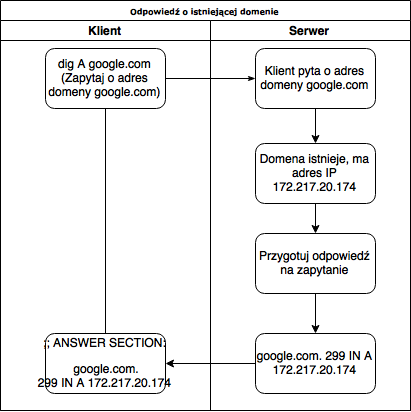
\includegraphics[scale=0.7]{image/nxdomain}
	\caption{Przepływ informacji podczas odpytywania serwera przestrzeni nazw o domenę.}
	\label{fig:dns_nxdomain}
	\end{figure}
\end{center}

Zarówno przypadek odpytywania o domenę istniejącą, jak i przypadek przeciwny zostały pokazane na schemacie \ref{fig:dns_nxdomain}.
Wyróżniono na nim stronę serwera oraz klienta oraz zaprezentowano części wiadomości, które są istotne dla konkretnego przypadku

Oba przytoczone powyżej przypadki są inaczej traktowane w protokole DNSSEC. Dla przykładu, gdy odpowiedzią jest
adres IP istniejącej domeny, serwer autorytatywny przechowuje określony, skończony zbiór podpisanych rekordów. Podpisy są tworzone
przy użyciu klucza prywatnego danej domeny. Istotny jest fakt, że podpisy rekordów nie są obliczane w czasie rzeczywistym, a jedynie
przechowywane razem z innymi rekordami w bazie danych DNS. Zaletą takiego rozwiązania jest oczywiście redukcja obliczeń wykonywanych
przez serwer autorytatywny a poza tym, tylko jeden z serwerów musi być w posiadaniu klucza prywatnego, więc dystrybucja klucza jest w
dużym stopniu uproszczona. Dodatkowo w przedstawionym wcześniej modelu nie ma potrzeby, aby weryfikować tożsamość każdego z serwerów
w systemie DNS, co ponownie upraszcza komunikację, zmniejsza obciążenie zasobów w sieci oraz ilość wymienianych informacji.

Problem listowania strefy DNS pojawia się wraz z charakterystyczną, negatywną odpowiedzią (w specyfikacji określaną jako NXDOMAIN).
Nie jest możliwe, aby odpowiadać na pytanie o niepoprawną domenę wcześniej przygotowaną wiadomością z obliczonym skrótem, ponieważ
może to prowadzić do skutecznego ataku powtórzeniowego (ang. \textit{reply attack}). Nie jest możliwe obliczenie wszystkich skrótów,
dla każdej z poddomen, bo takich przypadków jest zbyt wiele. Ciężko także zrezygnować z niewątpliwej zalety przytoczonej w poprzednim
akapicie -- braku konieczności obliczania skrótów w czasie rzeczywistym. Pomysłodawcy rozwiązania opisanego w RFC4034 \cite{RFC4034}
zaproponowali algorytm, dzięki któremu możliwe będzie utrzymanie substytutu podpisanej wiadomości NXDOMAIN. Cały system zachowuje
również zalety przedstawione w poprzednim akapicie. Rozwiązanie zakłada, że rekordy w strefie są uporządkowane, każda para rekordów
jest podpisana i tworzy rekord NSEC, a każdy rekord podpisany kluczem prywatnym. Jeśli serwer odbierze zapytanie o domenę, która
nie istnieje, odpowiada rekordem NSEC pary domen, które w uporządkowanej liście znajdują się odpowiednio przed i po odpytywanej
domenie oraz związane z nimi podpisy. Rozwiązanie zapewnia, że tylko serwer autorytatywny powinien być obdarzony zaufaniem oraz
umożliwia wstępną generację podpisów. Niestety wprowadza dodatkowo efekt uboczny, w postaci umożliwienia \textit{zone enumeration},
czyli wylistowania strefy. Przykładowa odpowiedź na zapytanie o nieistniejącą poddomenę została zaprezentwoana na listingu
\ref{list:dnssec_nx_domain}.

\begin{lstlisting}[label={list:dnssec_nx_domain},captionpos=b,caption=Odpowiedź na zapytanie DNSSEC o nieistniejącą domenę (na podstawie \cite{dnssec_nxdomain}).,language=bash]
$ kdig +dnssec +multiline ddadasds.example.com
;; ->>HEADER<<- opcode: QUERY; status: NXDOMAIN; id: 22793
;; Flags: qr aa rd; QUERY: 1; ANSWER: 0; AUTHORITY: 8; ADDITIONAL: 1
;; QUESTION SECTION:
;; ddadasds.example.com. IN A
;; AUTHORITY SECTION:
example.com. 3600 IN SOA dns1.example.com.
example.com. 3600 IN RRSIG SOA 13 2 3600 20170128184611
    ( 5134 example.com. nqiEgM+kVBDeBI== )
;; Matching record for hash of example.com;
0sc7qshrek878fcmnag1.example.com. 3600 IN NSEC3 1 0 0 AABB
    ( CPDHD7GK40NGDKRU8CQ8 NS SOA MX RRSIG DNSKEY NSEC3PARAM )
0sc7qshrek878fcmnag1.example.com. 3600 IN RRSIG NSEC3 13 3 3600
    ( 5134 example.com. 2JicIoTH3WkgAjbP/ehmTv== )
;; Covering record for hash of ddadasds.example.com;
jftj44t4kqppke20mukr.example.com. 3600 IN NSEC3 1 0 0 AABB
    ( MSC7QSHREK878FCM8GD7 A AAAA RRSIG )
jftj44t4kqppke20mukr.example.com. 3600 IN RRSIG NSEC3 13 3 3600
    ( 5134 example.com. VfFQfho5sQ8QVWOqsrXyN6== )
;; Covering record for hash of *.ddadasds.example.com;
cpdhd7gk40ngdkru8cq8n.example.com. 3600 IN NSEC3 1 0 0 AABB
    ( J1VSBFDBU38SMLNJPIMM A AAAA RRSIG )
cpdhd7gk40ngdkru8cq8n.example.com. 3600 IN RRSIG NSEC3 13 3 3600
    ( 5134 example.com. lcDsoeVGuq3rvezN2oW74x== )
;; Received 773 B
$
\end{lstlisting}

Zagadnienie listowania stref DNS samo w sobie często było podmiotem dyskusji. Początkowo wydano dokument, że nie jest to błędem,
że umożliwia się wypisanie bazy danych DNS \cite{RFC4033}. Później jednak wypracowany został kompromis \cite{RFC5155}, że w pewnych
przypadkach znajomość wszystkich domen może powodować dodatkowe niebezpieczeństwa. Przykłady, które przytoczono w RFC5155 \cite{RFC5155}
to na przykład dobre źródło danych wejściowych, które mogą posłużyć jako prawdopodobne adresy mailowe w kampaniach spamowych bądź
jako informacje o infrastrukturze wykorzystywane podczas rekonesansu DNS. Ponadto podatność nazywana \textit{zone enumeration}
może wpływać negatywnie na organizacje zajmujące się rejestrami DNS. Często są one zobowiązane do nieujawniania danych przechowywanych w
swoich rejestrach. Rekord NSEC umożliwia przeprowadzenie \textit{DNS enumeration} na strefach tych organizacji a następnie wykonanie
zapytań whois \cite{RFC3912} w celu pozyskania informacji o osobie rejestrującej domenę.
